

For all parts of this problem, I use Python as programming language. The part on incomplete markets is coded from scratch, and the parts on Arellano's debt default model builds on code found on Quantecon.

Codes and figures can be found in the project's \href{https://github.com/filipmellgren/QMM/tree/main/ps9}{Github repository}.

\section{Incomplete Markets Models with Aggregate Risk: KS VS BVK vs ABRS}

\subsection{Steady state}

I solve for the steady state in \texttt{incomplete\_markets.py}, where I find the following equilibrium objects:

\begin{itemize}
    \item Interest rate: \input{figures/ss_rate.txt}
    \item Capital: \input{figures/ss_capital.txt}
\end{itemize}

I solve for steady state using a bounded optimization algorithm that iterates on interest rates and return the squared error of market clearing as loss. Overall, this takes some minutes to solve for.

\subsection{Using BKM to find transition dynamics following a TFP shock}

For the TFP shock, I define a shock of 5\%, that decays at rate $\rho_A = 0.95$ over a $T = 150$ time horizon, assuming that the economy has returned sufficiently close to steady state after this passage of time. In the final period, I force $TFP_T = 1$.

As for variance and correlations with TFP, I find for $Y, K, C$ respectively the following:

\input{figures/corvar.txt}


\subsection{Comparing the above to second moments in the Krusell-Smith model}

For this part, I don't have the comparison with the KS-model unfortunately. Nontheless, the BKM gives the following figure of transition dynamics:

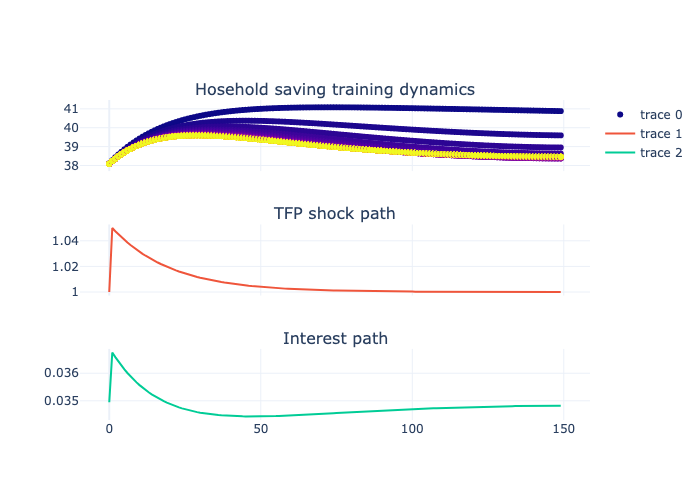
\includegraphics[scale = 0.8]{figures/training_dynamics.png}

In the top panel, I include training dynamics where color indicates iteration. Most visible paths are blue which indicate early iterations. The last iteration is yellow and largely overlaps other late paths.

The middle panel shows the exogenously defined TFP shock.

The bottom panel shows how interest rates evolve over the course of the shock.

It is interesting and intuitive to note that interest rates react fast, whereas it takes time for capital to peak, which again manages to bring down the interest rate. The sluggishness in response of capital can also be seen in its correlation with TFP, which is positively but rather low.

An issue I ran into when solving for this (note for future self), was that the ergodic distribution converged to the wrong distribution. We want the distribution associated with Eigenvalue 1, but there are several and these can appear if we iterate and make bad initial guesses. One simple check is to see whether uneployment corresponds to what we expect it to be.

\subsection{Compute impulse response using sequence space Jabobian method of Auclert et. al}

I am only starting to understand this fully so am not 100\% confident in these matrices yet. Nontheless, at this moment they appear as:

The Jacobian of the Household problem:

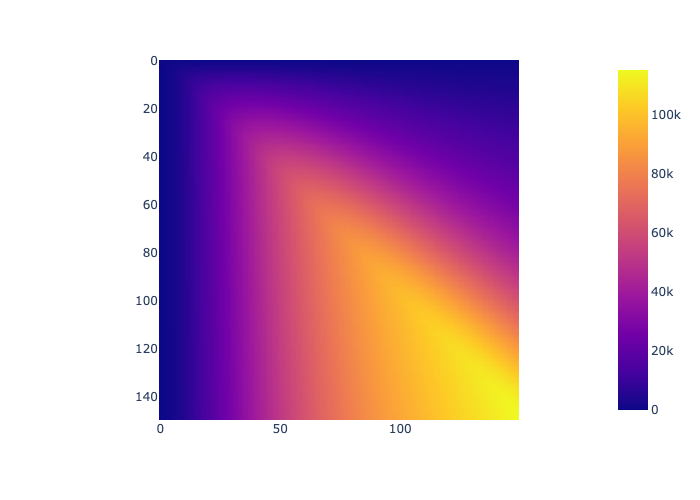
\includegraphics[scale = 0.75]{figures/jacobian.png}

The fake news matrix used to calculate the Jacobian:

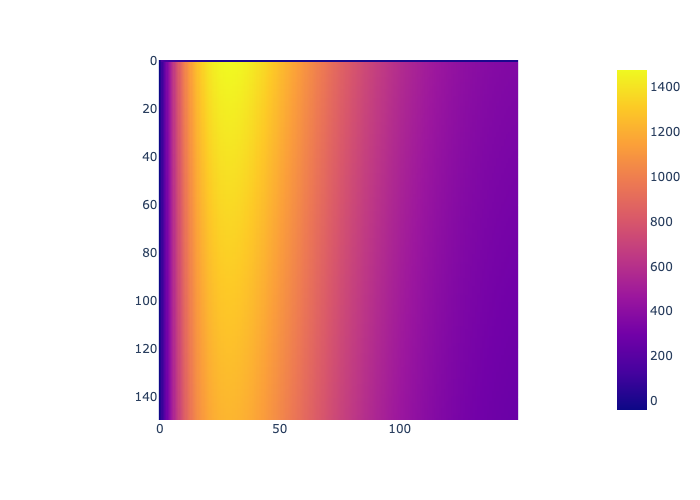
\includegraphics[scale = 0.75]{figures/fake_news.png}

\subsection{Larger shocks}

I provide a graph for a large shock that I solved for using the BKM method. I extended the time horizon until the economy has returned to steady state. Comparing the dynamics with the smaller shock, they look similar and it is hard to say whether there are nonlinearities present based on this. Perhaps the similarity suggests the method works, but I'd really want to compare with the full dynamic model to know for sure.

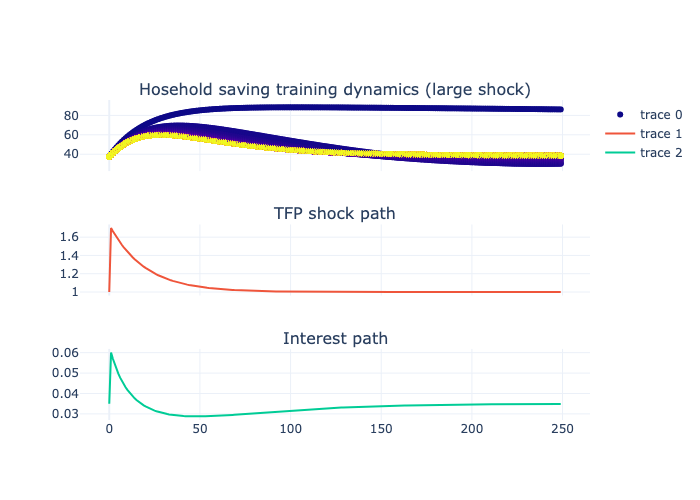
\includegraphics[scale = 0.8]{figures/training_dynamics_large_shock.png}

\section{Basic Arellano model}

For the Arellano model, I choose to build upon existing code available at \href{https://python-advanced.quantecon.org/arellano.html}{Quantecon}, which has a good explanation of the overall setup. My adapted code can be found in \texttt{arellano.py}

As for the Laffer curves, I am not sure they are correct. However, they tell us at which level of debt today that should not be exceeded.

The sovereign want to smooth consumption for its citizens in an economy that is exposed to shocks to production. The country is small and has no effect on capital markets so takes the interest rate as given. The sovereign can do so by choosing a level of debt, or to default and be locked out from capital markets for ever and ever. The advantage of defaulting is that costly debt does not need to be repaid. The drawback of a default is that the sovereign looses its ability to consumption smooth in the future. A more risk averse population would prefer to default later than a less risk averse population, as the former values the ability to smooth more than the later.

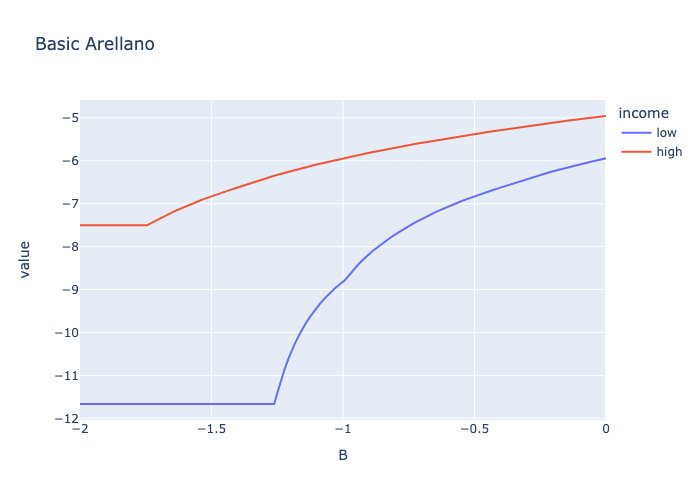
\includegraphics[scale = 0.75]{figures/basic_arellano.png}

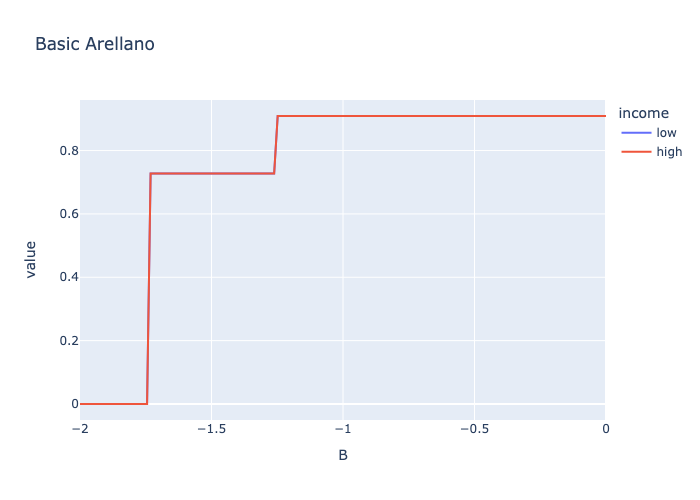
\includegraphics[scale = 0.75]{figures/basic_arellano_laffer.png}

We can see that if the economy is currently in a low income state, its threshold for whether to default is higher (more debt) than what it is if the economy is in a high income state. The interpretation is that the low income indebted sovereign can improve matters greatly today against a cost in the future. Since shocks are iid, the cost in the future is the same in the high income state, so the higher income needs to be offset by a higher debt for current affairs to be equally bad, and therefore as lucrative to default, as in the low income state. 

\section{Adding EV shocks to Arellano}

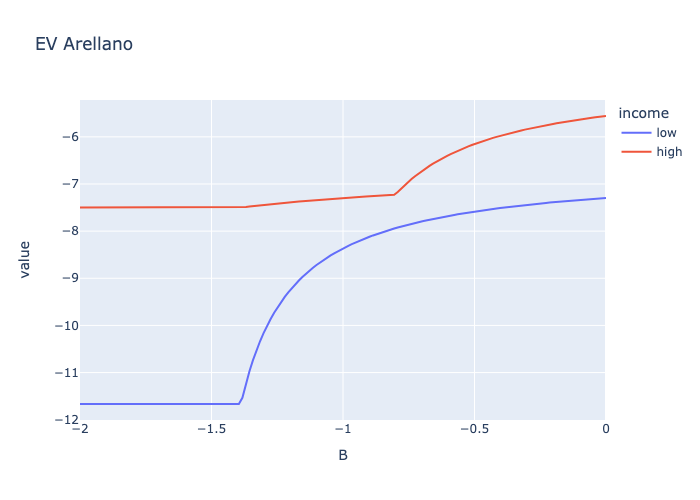
\includegraphics[scale = 0.75]{figures/EV_arellano.png}

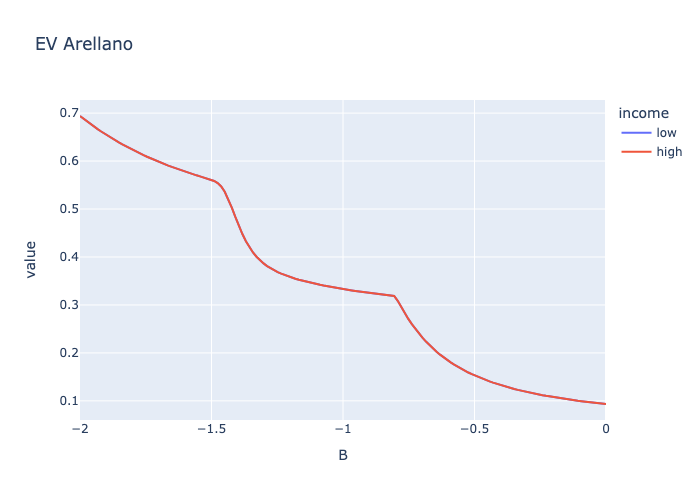
\includegraphics[scale = 0.75]{figures/EV_arellano_laffer.png}

With Extreme Value shocks, the choice to default becomes a probability, and curves become smooth..

\section{Solving Arellano with EV shocks using EGM}

I haven't solved this yet and prefer to spend more time learning about the Auclert et al framework before continuing with this.

